\part{Importing models}
\frame{\partpage}

\begin{frame}{Open Asset Import Library}
	\begin{itemize}
		\item There is an FBX SDK published by Autodesk, this can be used to load FBX files
		\pause\item We will use Asset Import Library to load FBX files
		\pause\item This allows us to support multiple file formats, including
		\begin{itemize}
			\pause\item FBX
			\pause\item OBJ 
			\pause\item DAE (aka Collada)
			\pause\item MD5 (DOOM3)
			\pause\item SMD (Half Life 2, Portal etc)
		\end{itemize}
	\end{itemize}
\end{frame}

\begin{frame}{Overview of an Assimp scene}
	\begin{center}
		\begin{figure}[h!]
			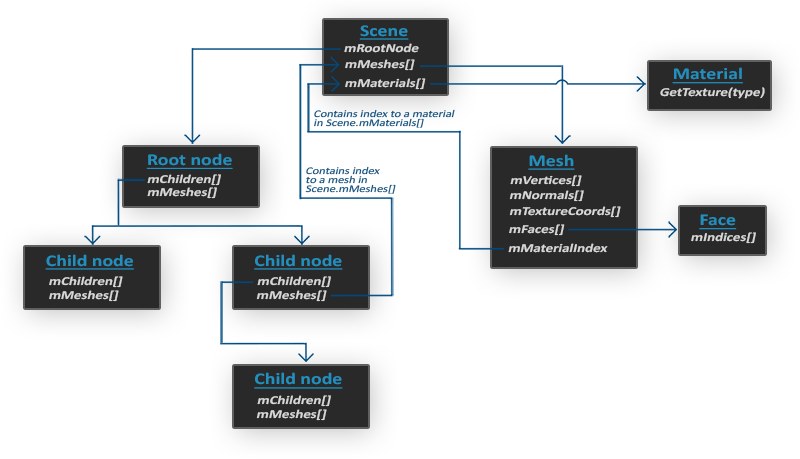
\includegraphics[width=\textwidth]{assimp_structure}
			\caption*{Image source: \url{https://learnopengl.com/Model-Loading/Assimp}}
		\end{figure}
	\end{center}
\end{frame}

\begin{frame}[fragile]{Loading a model from file}
		\begin{lstlisting}
Assimp::Importer importer;
const aiScene *scene = importer.ReadFile(path, flags); 
		\end{lstlisting}
		\begin{itemize}
		\pause\item An \href{http://assimp.sourceforge.net/lib_html/structai_scene.html}{\color{cyan}\lstinline{aiScene}} has (amongst other things):
		\begin{itemize}
			\pause\item \lstinline{aiMesh** mMeshes} - an array of pointers to the meshes in the scene
			\pause\item \lstinline{aiNode* mRootNode} - a pointer to the root node of the scene (provides access to all child nodes)
		\end{itemize}
		\pause\item An \href{http://assimp.sourceforge.net/lib_html/structai_node.html}{\color{cyan}\lstinline{aiNode}} has pointers to its \textbf{parent} and \textbf{child} nodes, the \textbf{indices} of its meshes, and a \textbf{transform} relative to its parent.
		\pause\item Optional \href{http://assimp.sourceforge.net/lib_html/postprocess_8h.html#a64795260b95f5a4b3f3dc1be4f52e410}{\color{cyan}\lstinline{flags}} can be supplied to specify post-processing steps, e.g. \lstinline{aiProcess_Triangulate}, \lstinline{aiProcess_GenNormals}
	\end{itemize} 
\end{frame}